%+TITLE: Lagrangianos relativistas
%+DESCRIPTION: Usando lo que hemos aprendido, construimos lagrangianos relativistas
\documentclass[11pt,a4paper]{article}

\usepackage[utf8]{inputenc}
\usepackage[T1]{fontenc}
\usepackage[spanish,es-nodecimaldot]{babel}
\usepackage{lmodern}
\usepackage{amsmath,amssymb,mathtools}
\usepackage{graphicx}
\usepackage{xcolor}
\usepackage{geometry}
\usepackage{enumitem}
\usepackage{microtype}

\geometry{margin=2.3cm}
\setlength{\parindent}{0pt}
\setlength{\parskip}{0.65em}
\setlist[itemize]{leftmargin=1.6em,itemsep=0.25em,topsep=0.25em}

\definecolor{title-red}{RGB}{165,25,20}
\definecolor{concept-green}{RGB}{20,125,45}
\newcommand{\concept}[1]{\textcolor{concept-green}{#1}}

\newcommand{\ket}[1]{\left|#1\right\rangle}
\newcommand{\bra}[1]{\left\langle#1\right|}
\newcommand{\braket}[2]{\left\langle #1\middle|#2\right\rangle}
\newcommand{\hc}{\mathrm{h.c.}}
\newcommand{\Tr}{\operatorname{Tr}}
\newcommand{\Diffs}{\mathrm{Diffs}}

\begin{document}

Ahora tenemos todas las piezas del rompecabezas. Queremos escribir el lagrangiano más general dados unos campos. Empezamos por el escalar.

Sabemos que para ser invariante de Lorentz, todos los índices deben estar contraídos. Se nos ocurre el siguiente lagrangiano:
\begin{align*}
  \mathcal L
  ={}&A_0+A_1\phi+A_2\phi^2+\cdots
     +B_0\Box\phi+B_1\phi\Box\phi+\cdots \\
    &+C_0\partial_\mu\phi\partial^\mu\phi
     +C_1\phi\partial_\mu\phi\partial^\mu\phi+\cdots.
\end{align*}

{\bf Podemos obviar $A_1$ escribiendo en términos de
$\widehat\phi=\phi-A_1/(2A_2)$, etc.}

{\bf El término $A_0$ no hace nada, por lo que $A_0=0$. El término $B_0$ es una derivada total, por lo que $B_0=0$.}

El término $B_1$ es redundante con $C_0$:
\begin{align*}
  \int d^4x\,\phi\Box\phi
  &=\int d^4x\left[
      \partial_\mu(\phi\partial^\mu\phi)
      -\partial_\mu\phi\partial^\mu\phi
    \right] \\
  &=\int_{\partial}d^3x\,\phi\partial^\mu\phi
    -\int d^4x\,\partial_\mu\phi\partial^\mu\phi.
\end{align*}
El primer término se anula si asumimos $\phi=0$ en el borde.

Entonces,
\[
  \mathcal L
  =A_2\phi^2+A_3\phi^3+A_4\phi^4+\cdots
   +B_1\phi\Box\phi+\cdots
   +C_0\partial_\mu\phi\partial^\mu\phi+\cdots.
\]

Ahora nos preguntamos por las unidades de las constantes. Es convención usual escoger unidades para el campo tales que $C_0=-1/2$. ¿Cuáles son las unidades de $\phi$ si hacemos eso?

\[
  [S]=Mv^2t=ML.
\]
En unidades naturales $\hbar=1$. Como
\[
  [\hbar]=ML,
  \qquad
  M=L^{-1},
\]
entonces
\[
  [S]=M^0.
\]
Además,
\[
  [\mathcal L]=L^{-4}[S]=M^4,
  \qquad
  [\partial_\mu]=L^{-1}=M.
\]
Como
\[
  [\partial_\mu\phi\partial^\mu\phi]=[\mathcal L]=M^4,
\]
obtenemos
\[
  [\phi]=M.
\]

Esto nos permite ahora escribir las unidades de cada término del lagrangiano. Lo escribimos de forma que las constantes sean adimensionales:
\begin{align*}
  \mathcal L={}&
  -\frac12(\partial_\mu\phi\partial^\mu\phi)
  +\frac{c_1}{M}\phi(\partial_\mu\phi\partial^\mu\phi)+\cdots
  +\frac{b_2}{M}\phi^2\Box\phi+\cdots \\
  &+\frac{d_0}{M^2}(\Box\phi)^2+\cdots
  +\frac{m^2}{2}\phi^2
  +\frac{\lambda_3}{3!}M\phi^3
  +\frac{\lambda_4}{4!}\phi^4
  +\frac{\lambda_5}{5!M}\phi^5+\cdots.
\end{align*}

Ahora bien, la cantidad $M$ tiene algún valor y dimensión de masa ($=$ energía). Si el sistema tiene una sola escala característica de energía, este $M$ debe ser esa escala. Recordemos además que en mecánica cuántica momento-energía son derivadas.

Si queremos describir este sistema para bajas energías $E\sim\partial_\mu\ll M$, tenemos
\[
  \mathcal L=-\frac12 f(\phi)
    (\partial_\mu\phi\partial^\mu\phi)+V(\phi).
\]

Además, en muchos casos excitar un campo requiere energía, tal que $\phi\ll M$, y nos quedamos con
\[
  \mathcal L
  =-\frac12\partial_\mu\phi\partial^\mu\phi
   -\frac{m^2}{2}\phi^2
   -\frac{\lambda_3M}{3!}\phi^3
   -\frac{\lambda_4}{4!}\phi^4.
\]

Usando Euler--Lagrange,
\[
  (\Box-m^2)\phi
  =\frac{\lambda_3}{2}M\phi^2
   +\frac{\lambda_4}{3!}\phi^3.
\]
Esta es la \concept{ecuación de Klein--Gordon} cuando $\lambda_3=0$ y $\lambda_4=0$.

Resolver esta ecuación es fácil cuando el lado derecho es cero:
\[
  -\ddot\phi+\nabla^2\phi-m^2\phi=0.
\]

Transformamos a Fourier,
\[
  \phi(t,\vec k)=\int d^3x\,e^{i\vec k\cdot\vec x}\phi(t,\vec x).
\]
Entonces,
\[
  \int d^3x\,e^{i\vec k\cdot\vec x}\ddot\phi(t,\vec x)
  =\int d^3x\,e^{i\vec k\cdot\vec x}
    (\nabla^2-m^2)\phi(t,\vec x),
\]
y
\[
  \ddot\phi(t,\vec k)
  =\left(\int d^3x\,e^{i\vec k\cdot\vec x}
      \nabla^2\phi(t,\vec x)\right)-m^2\phi(t,\vec k).
\]

Para el término entre paréntesis,
\begin{align*}
  \int d^3x\,e^{i\vec k\cdot\vec x}\nabla^2\phi(t,\vec x)
  &=\int d^3x\,\vec\nabla\cdot
      \left(e^{i\vec k\cdot\vec x}\vec\nabla\phi(t,\vec x)\right)
    -\int d^3x\,
      \left(\vec\nabla e^{i\vec k\cdot\vec x}\right)
      \cdot\vec\nabla\phi(t,\vec x) \\
  &=-i\int d^3x\,e^{i\vec k\cdot\vec x}
      \vec k\cdot\vec\nabla\phi(t,\vec x) \\
  &=-i\int d^3x\,\vec\nabla\cdot
      \left(\phi(t,\vec x)e^{i\vec k\cdot\vec x}\vec k\right)
    +i\int d^3x\,
      \vec k\cdot\left(\vec\nabla e^{i\vec k\cdot\vec x}\right)
      \phi(t,\vec x) \\
  &=-|\vec k|^2\int d^3x\,
      e^{i\vec k\cdot\vec x}\phi(t,\vec x)
   =-|\vec k|^2\phi(t,\vec k).
\end{align*}

Por tanto,
\[
  \ddot\phi(t,\vec k)
  =-(|\vec k|^2+m^2)\phi(t,\vec k)
  \equiv-\omega_k^2\phi(t,\vec k),
\]
y
\[
  \phi(t,\vec k)
  =a_k e^{i\omega_k t}+a_k^*e^{-i\omega_k t}.
\]

Los coeficientes $a_k$ estarán determinados por condiciones iniciales y la solución $\phi(t,\vec x)$ es la antitransformada de Fourier:
\[
  \phi(t,\vec x)
  =\int\frac{d^3k}{(2\pi)^3}e^{-i\vec k\cdot\vec x}
    \left(a_k e^{i\omega_k t}+a_k^*e^{-i\omega_k t}\right).
\]

Cada modo de Fourier se comporta como un oscilador con frecuencia
\[
  \omega_k=\sqrt{|\vec k|^2+m^2}.
\]

Para $|\vec k|\gg m$, $\omega\approx|\vec k|$ y cada modo es una onda plana de las de toda la vida. La información se propaga a velocidad $\omega/|\vec k|=1$.

Para $|\vec k|\ll m$, $\omega\approx m$ y cada modo tiene una velocidad de fase diferente,
\[
  \frac{\omega}{|\vec k|}\approx\frac{m}{|\vec k|}.
\]
En este caso la superposición de ondas tiende a perder coherencia y estar suprimida. Es decir, para distancias mayores que
\[
  L\sim\lambda\sim\frac1{|\vec k|}>\frac1m
\]
no hay propagación del campo.

Cuando $\lambda_3$ o $\lambda_4$ no son cero, no se sabe resolver exactamente la ecuación. En este caso se usa teoría de perturbaciones, asumiendo $\lambda_3\ll1$, $\lambda_4\ll1$. A estas perturbaciones se las llama ``interacciones''. La solución $\lambda_3=\lambda_4=0$ se llama ``libre''. Por ejemplo, con $\lambda_4\neq0$,
\[
  \ddot\phi_0-(m^2+\nabla^2)\phi_0=0,
\]
\[
  \ddot\phi_1-(m^2+\nabla^2)\phi_1
  =\frac{\lambda_4}{3!}\phi_0^3,
\]
\[
  \ddot\phi_2-(m^2+\nabla^2)\phi_2
  =\frac{\lambda_4}{2!}\phi_0^2\phi_1.
\]

\begin{figure}
  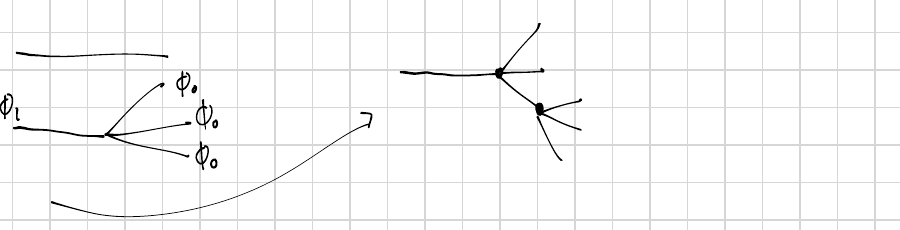
\includegraphics[width=0.78\linewidth]{figures/diagramas_perturbativos_phi4.png}
\end{figure}

\end{document}
